\documentclass[11pt,a4paper]{article}
\usepackage[margin=18mm,top=22mm,bottom=20mm]{geometry}
\usepackage{fontspec}\setmainfont{Latin Modern Roman}
\usepackage{xcolor}\usepackage{amsmath,amssymb,tikz,graphicx,fancyhdr,array,needspace}
\usetikzlibrary{patterns,arrows.meta,decorations.pathmorphing,calc}
\setlength{\headheight}{14pt}
\usetikzlibrary{arrows.meta}
\pagestyle{fancy}\fancyhf{}\renewcommand{\headrulewidth}{0.4pt}
\fancyhead[L]{\textbf{M-06}}\fancyhead[C]{\itshape Fizika — yechimlar (OliyFizika.uz)}\fancyhead[R]{\textbf{Mock №6}}
\fancyfoot[C]{\thepage}
\setlength{\parindent}{0pt}\setlength{\parskip}{3pt}
\newcommand{\opt}[2]{\hspace*{4mm}#1)\ #2\par}
\newcommand{\blank}{\rule{5cm}{0.4pt}}
\begin{document}

\begin{center}{\Large\textbf{FIZIKA — YECHIMLAR}}\\[2pt]{\large Mock №6}\end{center}
\Needspace{10\baselineskip}\noindent\begin{minipage}{\linewidth}
\textbf{1.}\ 350 g massali koptok 4 m balandlikka otildi. Uning maksimal potensial energiyasini (J) aniqlang.\par\smallskip
\opt{A}{7}
\opt{B}{10}
\opt{C}{14}
\opt{D}{18}
\end{minipage}\vspace{2pt}\par
\noindent\colorbox{gray!12}{\parbox{\dimexpr\linewidth-2\fboxsep}{\textbf{Javob: C) 14}}}\par\smallskip
\noindent\textit{Yechim.}\ $E_p=mgh=0{,}35\cdot10\cdot4=14$ J.\par\par\medskip\hrule\medskip
\Needspace{10\baselineskip}\noindent\begin{minipage}{\linewidth}
\textbf{2.}\ Qözğalmas blok orqali ötkazilgan arqonning uçlariga 50 g va 75 g yuklar osilgan. Arqon va blok massasi hisobga olinmaydigan darajada kiçik. Arqonni çözilmas deb olib, yuklarning harakatlaniş tezlanişini (m/s$^{2}$) va arqonning taranglik kuçini toping (N). g=9,8 N/kg.\par\smallskip
\opt{A}{1,96; 0,6}
\opt{B}{1,96; 1,2}
\opt{C}{1,96; 0,3}
\opt{D}{2; 0,6}
\end{minipage}\vspace{2pt}\par
\noindent\colorbox{gray!12}{\parbox{\dimexpr\linewidth-2\fboxsep}{\textbf{Javob: A) 1,96; 0,6}}}\par\smallskip
\noindent\textit{Yechim.}\ \[a=\frac{(m_2-m_1)g}{m_1+m_2}=\frac{0{,}025\cdot9{,}8}{0{,}125}=1{,}96\ \text{m/s}^2,\qquad T=m_1(g+a)=0{,}05\cdot11{,}76\approx0{,}6\ \text{N}.\]\par\medskip\hrule\medskip
\Needspace{10\baselineskip}\noindent\begin{minipage}{\linewidth}
\textbf{3.}\ Nima uçun zilzila payti odam yer qimirlaşini 2 marta sezadi?\par\smallskip
\opt{A}{çunki, zil zila markazidan odamga böylama tölqin birinçi bölib yetib keladi}
\opt{B}{çunki, zil zila markazidan odamga köndalang tölqin birinçi bölib yetib keladi}
\opt{C}{çunki, zil zila markazidan odamga böylama va köndalang tölqin bir vaqtda yetib keladi}
\opt{D}{bunday hodisa kuzatilmaydi}
\end{minipage}\vspace{2pt}\par
\noindent\colorbox{gray!12}{\parbox{\dimexpr\linewidth-2\fboxsep}{\textbf{Javob: A) çunki, zil zila markazidan odamga böylama tölqin birinçi bölib yetib keladi}}}\par\smallskip
\noindent\textit{Yechim.}\ Zilzila öçoğidan böylama va köndalang tölqinlar tarqaladi. Böylama tölqin tezroq, u birinçi yetib keladi; keyin köndalang tölqin keladi. Şuning uçun silkiniş ikki marta seziladi.\par\par\medskip\hrule\medskip
\Needspace{10\baselineskip}\noindent\begin{minipage}{\linewidth}
\textbf{4.}\ Jism birinçi marta gorizontga 60$^\circ$ burçak ostida, ikkinçi marta gorizontga 30$^\circ$ burçak ostida otildi. Birinçi marta otilganda jism neça marta balandroqqa kötariladi, agarda birinçi marta jism otilganda ikki marta uzoqroqqa borib tuşgan bölsa? g=10 m/s$^{2}$.\par\smallskip
\opt{A}{4}
\opt{B}{5}
\opt{C}{6}
\opt{D}{8}
\end{minipage}\vspace{2pt}\par
\noindent\colorbox{gray!12}{\parbox{\dimexpr\linewidth-2\fboxsep}{\textbf{Javob: C) 6}}}\par\smallskip
\noindent\textit{Yechim.}\ $L=\frac{v^2\sin2\alpha}{g}$, $H=\frac{v^2\sin^2\alpha}{2g}$. $\sin120^\circ=\sin60^\circ$, demak $\frac{L_1}{L_2}=\frac{v_1^2}{v_2^2}=2$.\par
\[\frac{H_1}{H_2}=\frac{v_1^2\sin^260^\circ}{v_2^2\sin^230^\circ}=2\cdot\frac{3/4}{1/4}=6.\]\par\medskip\hrule\medskip
\Needspace{10\baselineskip}\noindent\begin{minipage}{\linewidth}
\textbf{5.}\ Bikrligi 1,6 kN/m bölgan purjinaga 5 kg osilgan. Purjina qançaga (sm) çöziladi?\par\smallskip
\opt{A}{8/25}
\opt{B}{12/5}
\opt{C}{25/8}
\opt{D}{16/5}
\end{minipage}\vspace{2pt}\par
\noindent\colorbox{gray!12}{\parbox{\dimexpr\linewidth-2\fboxsep}{\textbf{Javob: C) 25/8}}}\par\smallskip
\noindent\textit{Yechim.}\ $x=\frac{mg}{k}=\frac{50}{1600}$ m $=\frac{5000}{1600}$ cm $=\frac{25}{8}$ cm.\par\par\medskip\hrule\medskip
\Needspace{10\baselineskip}\noindent\begin{minipage}{\linewidth}
\textbf{6.}\ Jism 3,2 m balandlikdan boşlanğiç tezliksiz taşlandi. Şu vaqtda birinçi jism urilişidagi tezligidan 1,5 marta kiçik tezlik bilan ikkinçi jism yerdan yuqoriga otilgan. Ular qanday balandlikda (cm) uçraşadilar? g=10 m/s$^{2}$.\par\smallskip
\opt{A}{320}
\opt{B}{100}
\opt{C}{140}
\opt{D}{160}
\end{minipage}\vspace{2pt}\par
\noindent\colorbox{gray!12}{\parbox{\dimexpr\linewidth-2\fboxsep}{\textbf{Javob: C) 140}}}\par\smallskip
\noindent\textit{Yechim.}\ Birinçi jismning yerga uriliş tezligi $v_1=\sqrt{2gH}=8$ m/s, ikkinçisining boşlanğiç tezligi $v_2=8/1{,}5=16/3$ m/s. Ikkala jism bir xil tezlanişda, nisbiy tezlik $v_2$ özgarmas:\par
\[t=\frac{H}{v_2}=\frac{3{,}2}{16/3}=0{,}6\ \text{s},\qquad h=H-\frac{gt^2}{2}=3{,}2-1{,}8=1{,}4\ \text{m}=140\ \text{cm}.\]\par\medskip\hrule\medskip
\Needspace{10\baselineskip}\noindent\begin{minipage}{\linewidth}
\textbf{7.}\ Moddiy nuqtaning koordinatalari x = 3t [m], y = 4t [m] va = 0 [m] qonuniyatlarga böysunadi. Moddiy nuqtaning 5 s dagi köçiş modulini toping (m).\par\smallskip
\opt{A}{10}
\opt{B}{15}
\opt{C}{25}
\opt{D}{20}
\end{minipage}\vspace{2pt}\par
\noindent\colorbox{gray!12}{\parbox{\dimexpr\linewidth-2\fboxsep}{\textbf{Javob: C) 25}}}\par\smallskip
\noindent\textit{Yechim.}\ 5 s da $x=15$ m, $y=20$ m: $s=\sqrt{15^2+20^2}=25$ m.\par\par\medskip\hrule\medskip
\Needspace{10\baselineskip}\noindent\begin{minipage}{\linewidth}
\textbf{8.}\ Suvga limmo-lim töldirilgan idişga 800 kg/m$^{3}$ ziçlikli jism taşlansa, qanday hajmli suv idişdan tökiladi (m$^{3}$)? Jismning hajmi 2 m$^{3}$ ga teng.\par\smallskip
\opt{A}{1,2}
\opt{B}{2}
\opt{C}{1,4}
\opt{D}{1,6}
\end{minipage}\vspace{2pt}\par
\noindent\colorbox{gray!12}{\parbox{\dimexpr\linewidth-2\fboxsep}{\textbf{Javob: D) 1,6}}}\par\smallskip
\noindent\textit{Yechim.}\ Jism ziçligi suvnikidan kiçik — u suzadi. Siqib çiqarilgan suv massasi jism massasiga teng:\par
\[V_s=\frac{\rho V}{\rho_s}=\frac{800\cdot2}{1000}=1{,}6\ \text{m}^3.\]\par\medskip\hrule\medskip
\Needspace{10\baselineskip}\noindent\begin{minipage}{\linewidth}
\textbf{9.}\ Arava 120 kN kuç ta’siri ostida 2,3 km masofa bosgan bölsa, qança (MJ) iş bajargan?\par\smallskip
\opt{A}{49600}
\opt{B}{1860}
\opt{C}{276}
\opt{D}{683}
\end{minipage}\vspace{2pt}\par
\noindent\colorbox{gray!12}{\parbox{\dimexpr\linewidth-2\fboxsep}{\textbf{Javob: C) 276}}}\par\smallskip
\noindent\textit{Yechim.}\ $A=Fs=120\cdot10^3\cdot2300=2{,}76\cdot10^8$ J $=276$ MJ.\par\par\medskip\hrule\medskip
\Needspace{10\baselineskip}\noindent\begin{minipage}{\linewidth}
\textbf{10.}\ Jism 120 m balandlikdan gorizontal otildi. Bundan 4 s ötgan paytda uning tezlik vektori gorizont bilan 45$^\circ$ burçak hosil qildi. U qanday tezlik bilan otilgan (m/s)? g=10 m/s$^{2}$.\par\smallskip
\opt{A}{25}
\opt{B}{30}
\opt{C}{40}
\opt{D}{45}
\end{minipage}\vspace{2pt}\par
\noindent\colorbox{gray!12}{\parbox{\dimexpr\linewidth-2\fboxsep}{\textbf{Javob: C) 40}}}\par\smallskip
\noindent\textit{Yechim.}\ 4 s dan keyin $v_y=gt=40$ m/s. $45^\circ$ da $v_x=v_y$, demak $v_0=40$ m/s.\par\par\medskip\hrule\medskip
\Needspace{10\baselineskip}\noindent\begin{minipage}{\linewidth}
\textbf{11.}\ Agar har 10 m balandlikda atmosfera bosimi 1 mm.Hg ga kamayadigan bölsa, dengiz sathidan 4,6 km balandlikdagi havoning 1 cm$^{3}$ hajmida qança molekula böladi? Dengiz sathida atmosfera bosimi 760 mm.Hg ga teng. Havo harorati 27 $^\circ$C. Haroratning balandlik böyiça özgarişini hisobga olmang. 1 mm.Hg=133,3 Pa.\par\smallskip
\opt{A}{9,66$\cdot10^{17}$}
\opt{B}{4,66$\cdot10^{15}$}
\opt{C}{9,66$\cdot10^{20}$}
\opt{D}{9,66$\cdot10^{18}$}
\end{minipage}\vspace{2pt}\par
\noindent\colorbox{gray!12}{\parbox{\dimexpr\linewidth-2\fboxsep}{\textbf{Javob: D) 9,66$\cdot10^{18}$}}}\par\smallskip
\noindent\textit{Yechim.}\ Bosimning kamayişi $4600/10=460$ mm.Hg, ya’ni $p=300$ mm.Hg $=300\cdot133{,}3\approx4\cdot10^4$ Pa.\par
\[n=\frac{p}{kT}=\frac{39\,990}{1{,}38\cdot10^{-23}\cdot300}\approx9{,}66\cdot10^{24}\ \text{m}^{-3}=9{,}66\cdot10^{18}\ \text{cm}^{-3}.\]\par\medskip\hrule\medskip
\Needspace{10\baselineskip}\noindent\begin{minipage}{\linewidth}
\textbf{12.}\ Gaz ballon içidagi barometr gaz bosimi 10 atm ekanini körsatdi. Ballonga ulangan manometr körsatişini toping (atm).\par\smallskip
\opt{A}{9}
\opt{B}{10}
\opt{C}{11}
\opt{D}{20}
\end{minipage}\vspace{2pt}\par
\noindent\colorbox{gray!12}{\parbox{\dimexpr\linewidth-2\fboxsep}{\textbf{Javob: A) 9}}}\par\smallskip
\noindent\textit{Yechim.}\ Manometr atmosfera bosimidan ortiqça bosimni körsatadi: $10-1=9$ atm.\par\par\medskip\hrule\medskip
\Needspace{10\baselineskip}\noindent\begin{minipage}{\linewidth}
\textbf{13.}\ Gazning bitta molekulasi massasi $7{,}3\cdot10^{-26}$ kg. Bu qanday gaz? $N_A=6{,}02\cdot10^{23}$ mol$^{-1}$.\par\smallskip
\opt{A}{$N_2$}
\opt{B}{$O_2$}
\opt{C}{$CO_2$}
\opt{D}{$O_3$}
\end{minipage}\vspace{2pt}\par
\noindent\colorbox{gray!12}{\parbox{\dimexpr\linewidth-2\fboxsep}{\textbf{Javob: C) $CO_2$}}}\par\smallskip
\noindent\textit{Yechim.}\ $M=m_0N_A=7{,}3\cdot10^{-26}\cdot6{,}02\cdot10^{23}\approx0{,}044$ kg/mol — bu $CO_2$ ($12+2\cdot16=44$).\par\par\medskip\hrule\medskip
\Needspace{10\baselineskip}\noindent\begin{minipage}{\linewidth}
\textbf{14.}\ Hajmi 8,31 m$^{3}$ bölgan ballon har sekundda 2 g dan vodorod gazi bilan töldirilmoqda. Ballondagi bosimni 1,8$\cdot10^{5}$ Pa ga yetkaziş uçun qança vaqt kerak böladi (min)? Gazni temperaturasi 27 $^\circ$C ga teng.\par\smallskip
\opt{A}{10}
\opt{B}{8}
\opt{C}{5}
\opt{D}{1,8}
\end{minipage}\vspace{2pt}\par
\noindent\colorbox{gray!12}{\parbox{\dimexpr\linewidth-2\fboxsep}{\textbf{Javob: A) 10}}}\par\smallskip
\noindent\textit{Yechim.}\ \[\nu=\frac{pV}{RT}=\frac{1{,}8\cdot10^5\cdot8{,}31}{8{,}31\cdot300}=600\ \text{mol},\qquad m=1200\ \text{g}.\]
Vaqt $t=1200/2=600$ s $=10$ min.\par\par\medskip\hrule\medskip
\Needspace{10\baselineskip}\noindent\begin{minipage}{\linewidth}
\textbf{15.}\ Ideal gazning hajmi $V$ ga, konsentratsiyasi $n$ ga teng. Agar har bir gaz molekulasi örtaça $\bar{E}_k$ kinetik energiyaga ega bölsa, gazning içki energiyasini aniqlang.\par\smallskip
\opt{A}{$\dfrac{\bar{E}_k}{nV}$}
\opt{B}{$nV\bar{E}_k$}
\opt{C}{$\dfrac{V\bar{E}_k}{n}$}
\opt{D}{$\dfrac{n\bar{E}_k}{V}$}
\end{minipage}\vspace{2pt}\par
\noindent\colorbox{gray!12}{\parbox{\dimexpr\linewidth-2\fboxsep}{\textbf{Javob: B) $nV\bar{E}_k$}}}\par\smallskip
\noindent\textit{Yechim.}\ Molekulalar soni $N=nV$, ideal gaz içki energiyasi barça molekulalar kinetik energiyalari yiğindisi: $U=nV\bar E_k$.\par\par\medskip\hrule\medskip
\Needspace{10\baselineskip}\noindent\begin{minipage}{\linewidth}
\textbf{16.}\ Massasi 200 g bölgan magnit vertikal pölat devorga 2 N kuç bilan yopişib turibdi. Agar işqalaniş koeffitsiyenti 0,2 ga teng bölsa, magnitni devor böylab yuqoriga tekis harakatlantiriş uçun qanday kuç kerak böladi (N)? g=10 N/kg.\par\smallskip
\opt{A}{2}
\opt{B}{3,2}
\opt{C}{5,2}
\opt{D}{2,4}
\end{minipage}\vspace{2pt}\par
\noindent\colorbox{gray!12}{\parbox{\dimexpr\linewidth-2\fboxsep}{\textbf{Javob: D) 2,4}}}\par\smallskip
\noindent\textit{Yechim.}\ Normal bosim kuçi $N=2$ N, işqalaniş $\mu N=0{,}4$ N. Tekis kötariş uçun $F=mg+\mu N=2+0{,}4=2{,}4$ N.\par\par\medskip\hrule\medskip
\Needspace{10\baselineskip}\noindent\begin{minipage}{\linewidth}
\textbf{17.}\ Siğimlari $C_1 = 2C_2 = 3C_3$ bölgan kondensatorlar özgarmas kuçlaniş manbayiga ketma-ket ulangan. Ularda töplanadigan zaryad miqdorlarini taqqoslang.\par\smallskip
\opt{A}{$q_1 = 2q_2 = 3q_3$}
\opt{B}{$q_1 = q_2 = q_3$}
\opt{C}{$3q_1 = 2q_2 = q_3$}
\opt{D}{$q_1 = 4q_2 = 9q_3$}
\end{minipage}\vspace{2pt}\par
\noindent\colorbox{gray!12}{\parbox{\dimexpr\linewidth-2\fboxsep}{\textbf{Javob: B) $q_1 = q_2 = q_3$}}}\par\smallskip
\noindent\textit{Yechim.}\ Ketma-ket ulangan kondensatorlarda zaryadlar bir xil: $q_1=q_2=q_3$.\par\par\medskip\hrule\medskip
\Needspace{10\baselineskip}\noindent\begin{minipage}{\linewidth}
\textbf{18.}\ Çeksiz uzunlikdagi ötkazgiçdan $10\pi$ A tok ötmoqda. Ötkazgiçdan 2 m naridagi magnit maydon kuçlanganligi (A/m) va induksiyasini toping (T).\par\smallskip
\opt{A}{$2{,}5;\ \pi\cdot10^{-6}$}
\opt{B}{$2{,}5;\ \pi\cdot10^{-5}$}
\opt{C}{$5;\ \pi\cdot10^{-6}$}
\opt{D}{$2;\ \pi\cdot10^{-6}$}
\end{minipage}\vspace{2pt}\par
\noindent\colorbox{gray!12}{\parbox{\dimexpr\linewidth-2\fboxsep}{\textbf{Javob: A) $2{,}5;\ \pi\cdot10^{-6}$}}}\par\smallskip
\noindent\textit{Yechim.}\ \[H=\frac{I}{2\pi r}=\frac{10\pi}{4\pi}=2{,}5\ \text{A/m},\qquad B=\mu_0H=4\pi\cdot10^{-7}\cdot2{,}5=\pi\cdot10^{-6}\ \text{T}.\]\par\medskip\hrule\medskip
\Needspace{10\baselineskip}\noindent\begin{minipage}{\linewidth}
\textbf{19.}\ Ampermetrning ölçaş çegarasini oşiriş maqsadida unga şunt $\ldots$ ulanadi, şuntning qarşiligi esa ampermetrning qarşiligidan $\ldots$ böladi. Nuqtalar örnini töldiring.\par\smallskip
\opt{A}{ketma-ket, katta}
\opt{B}{ketma-ket, kiçik}
\opt{C}{parallel, katta}
\opt{D}{parallel, kiçik}
\end{minipage}\vspace{2pt}\par
\noindent\colorbox{gray!12}{\parbox{\dimexpr\linewidth-2\fboxsep}{\textbf{Javob: D) parallel, kiçik}}}\par\smallskip
\noindent\textit{Yechim.}\ Şunt ampermetrga parallel ulanadi va tokning asosiy qismini ötkazişi uçun uning qarşiligi ampermetrnikidan kiçik böladi.\par\par\medskip\hrule\medskip
\Needspace{10\baselineskip}\noindent\begin{minipage}{\linewidth}
\textbf{20.}\ Zaryadlari $-$5e va +3e bölgan suv tomçilari birlaştirilsa, qanday zaryadli tomçi hosil böladi? e – elementar zaryad.\par\smallskip
\opt{A}{$-$2e}
\opt{B}{$-$4e}
\opt{C}{+2e}
\opt{D}{+4e}
\end{minipage}\vspace{2pt}\par
\noindent\colorbox{gray!12}{\parbox{\dimexpr\linewidth-2\fboxsep}{\textbf{Javob: A) $-$2e}}}\par\smallskip
\noindent\textit{Yechim.}\ Zaryadning saqlaniş qonuni: $-5e+3e=-2e$.\par\par\medskip\hrule\medskip
\Needspace{10\baselineskip}\noindent\begin{minipage}{\linewidth}
\textbf{21.}\ Ikki kislorod ioni berilgan. Birinçisi bitta, ikkinçisi ikkita elektron yöqotgan. Ular bir jinsli magnit maydonga bir xil tezlik bilan induksiya çiziqlariga tik ravişda uçib kirişsa, birinçi va ikkinçi ionlar harakat trayektoriyasining radiuslari $r_1$ va $r_2$ orasidagi munosabat qanday böladi?\par\smallskip
\opt{A}{$r_1$=4$r_2$}
\opt{B}{$r_1$=2$r_2$}
\opt{C}{2$r_1$=$r_2$}
\opt{D}{4$r_1$=$r_2$}
\end{minipage}\vspace{2pt}\par
\noindent\colorbox{gray!12}{\parbox{\dimexpr\linewidth-2\fboxsep}{\textbf{Javob: B) $r_1$=2$r_2$}}}\par\smallskip
\noindent\textit{Yechim.}\ $r=\frac{mv}{qB}$; massalar va tezliklar bir xil, $q_2=2q_1$, demak $r_1=2r_2$.\par\par\medskip\hrule\medskip
\Needspace{10\baselineskip}\noindent\begin{minipage}{\linewidth}
\textbf{22.}\ 10 A tokka ulangan sterjen gorizontal holatda ikkita bir xil prujinaga osib qöyildi. Agar sterjen perpendikulyar magnit maydonda joylaşgan bölsa, prujinalarning çözilişini toping (cm). Sterjen uzunligi 20 cm. g=10 m/s$^{2}$.\par\smallskip
\noindent\hspace*{4mm}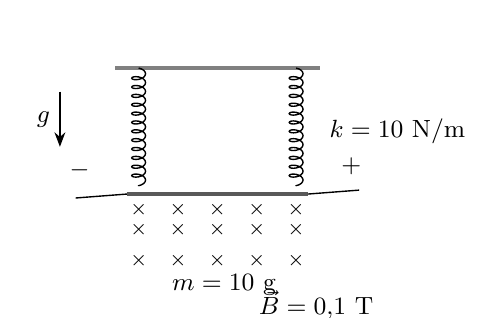
\begin{tikzpicture}[x=1cm,y=1cm,line width=0.5pt,>=Stealth,font=\small]
\draw[line width=1.2pt,gray] (0,3.0)--(2.6,3.0);
\draw[decorate,decoration={coil,aspect=0.5,segment length=3.2,amplitude=2.5}] (0.3,3.0)--(0.3,1.5);
\draw[decorate,decoration={coil,aspect=0.5,segment length=3.2,amplitude=2.5}] (2.3,3.0)--(2.3,1.5);
\draw[line width=1.6pt,gray!70!black] (0.15,1.4)--(2.45,1.4);
\foreach \x in {0.3,0.8,1.3,1.8,2.3}{\foreach \y in {0.55,0.95,1.2}{\node[font=\scriptsize] at (\x,\y) {$\times$};}}
\draw (-0.5,1.35)--(0.15,1.4); \draw (2.45,1.4)--(3.1,1.45); \node at (-0.45,1.7) {$-$}; \node at (3.0,1.75) {$+$};
\node[below right] at (0.6,0.5) {$m=10\ \mathrm{g}$}; \node[below right] at (1.7,0.3) {$\vec B=0{,}1\ \mathrm{T}$};
\draw[->] (-0.7,2.7)--(-0.7,2.0) node[midway,left]{$g$}; \node[right] at (2.6,2.2) {$k=10\ \mathrm{N/m}$};
\end{tikzpicture}\par\smallskip
\opt{A}{3}
\opt{B}{1,5}
\opt{C}{2}
\opt{D}{0,5}
\end{minipage}\vspace{2pt}\par
\noindent\colorbox{gray!12}{\parbox{\dimexpr\linewidth-2\fboxsep}{\textbf{Javob: B) 1,5}}}\par\smallskip
\noindent\textit{Yechim.}\ Tok «+» dan «$-$» ga, ya’ni öngdan çapga oqadi; induksiya çizma tekisligidan içkariga. Çap qöl qoidasiga köra Amper kuçi pastga yönalgan: $F_A=BIL=0{,}1\cdot10\cdot0{,}2=0{,}2$ N. Muvozanat: $2kx=mg+F_A=0{,}1+0{,}2=0{,}3$ N,\par
\[x=\frac{0{,}3}{2\cdot10}=0{,}015\ \text{m}=1{,}5\ \text{cm}.\]\par\medskip\hrule\medskip
\Needspace{10\baselineskip}\noindent\begin{minipage}{\linewidth}
\textbf{23.}\ Özgaruvçan tok zanjirida tok kuçining maksimal qiymati 18 mA ga, zaryadning maksimal qiymati esa 0,03 $\mu$C ga teng. Konturning tebraniş davri ($\mu$s) aniqlansin. $\pi$ = 3.\par\smallskip
\opt{A}{10}
\opt{B}{5}
\opt{C}{15}
\opt{D}{20}
\end{minipage}\vspace{2pt}\par
\noindent\colorbox{gray!12}{\parbox{\dimexpr\linewidth-2\fboxsep}{\textbf{Javob: A) 10}}}\par\smallskip
\noindent\textit{Yechim.}\ $I_0=q_0\omega$: $\omega=\frac{18\cdot10^{-3}}{3\cdot10^{-8}}=6\cdot10^5$ rad/s.\par
\[T=\frac{2\pi}{\omega}=\frac{6}{6\cdot10^5}=10^{-5}\ \text{s}=10\ \mu\text{s}.\]\par\medskip\hrule\medskip
\Needspace{10\baselineskip}\noindent\begin{minipage}{\linewidth}
\textbf{24.}\ Akkumulyator 60 A$\cdot$h zaryad töplagan. Bu neça kulon böladi?\par\smallskip
\opt{A}{54000}
\opt{B}{27000}
\opt{C}{108000}
\opt{D}{216000}
\end{minipage}\vspace{2pt}\par
\noindent\colorbox{gray!12}{\parbox{\dimexpr\linewidth-2\fboxsep}{\textbf{Javob: D) 216000}}}\par\smallskip
\noindent\textit{Yechim.}\ $q=60\ \text{A}\cdot3600\ \text{s}=216\,000$ C.\par\par\medskip\hrule\medskip
\Needspace{10\baselineskip}\noindent\begin{minipage}{\linewidth}
\textbf{25.}\ Uzunliklarining nisbati $l_2/l_1=2$, köndalang kesimlarining nisbati $S_1/S_2=2$ bölgan, bir xil materialdan tayyorlangan ikkita ötkazgiçga bir xil kuçlaniş berilsa, ulardagi tok ziçliklari qanday munosabatda böladi?\par\smallskip
\opt{A}{$j_1=j_2/2$}
\opt{B}{$j_1=4j_2$}
\opt{C}{$j_1=j_2$}
\opt{D}{$j_1=2j_2$}
\end{minipage}\vspace{2pt}\par
\noindent\colorbox{gray!12}{\parbox{\dimexpr\linewidth-2\fboxsep}{\textbf{Javob: D) $j_1=2j_2$}}}\par\smallskip
\noindent\textit{Yechim.}\ $j=\frac{I}{S}=\frac{U}{RS}=\frac{U}{\rho l}$ — tok ziçligi kesim yuzasiga boğliq emas. $l_2=2l_1$ bölgani uçun $j_1=2j_2$.\par\par\medskip\hrule\medskip
\Needspace{10\baselineskip}\noindent\begin{minipage}{\linewidth}
\textbf{26.}\ Fokus masofasi 10 cm bölgan yiğuvçi linzada buyumning tasviri hosil qilinmoqda. Buyum linzadan 5 cm masofada turibdi. Agar buyumni linzadan 10 cm ga uzoqlaştirsak uning tasviri qançaga (cm) siljiydi?\par\smallskip
\opt{A}{20}
\opt{B}{35}
\opt{C}{25}
\opt{D}{40}
\end{minipage}\vspace{2pt}\par
\noindent\colorbox{gray!12}{\parbox{\dimexpr\linewidth-2\fboxsep}{\textbf{Javob: D) 40}}}\par\smallskip
\noindent\textit{Yechim.}\ $d_1=5$ cm $<F$: $\frac1{f_1}=\frac1{10}-\frac15=-\frac1{10}$ — mavhum tasvir linzadan 10 cm (buyum tomonda). $d_2=15$ cm: $\frac1{f_2}=\frac1{10}-\frac1{15}=\frac1{30}$ — haqiqiy tasvir narigi tomonda 30 cm da. Tasvir $10+30=40$ cm ga siljiydi.\par\par\medskip\hrule\medskip
\Needspace{10\baselineskip}\noindent\begin{minipage}{\linewidth}
\textbf{27.}\ Nuqta fokus masofasi 20 cm bölgan yupqa yiğuvçi linzaning boş optik öqidan 1 cm balandlikda turibdi. Nuqta va linza orasidagi masofa 25 cm. Uning tasviri bu öqdan qanday masofada (cm) hosil bölgan?\par\smallskip
\opt{A}{1}
\opt{B}{2}
\opt{C}{4}
\opt{D}{3}
\end{minipage}\vspace{2pt}\par
\noindent\colorbox{gray!12}{\parbox{\dimexpr\linewidth-2\fboxsep}{\textbf{Javob: C) 4}}}\par\smallskip
\noindent\textit{Yechim.}\ $f=\frac{dF}{d-F}=\frac{25\cdot20}{5}=100$ cm, $\Gamma=f/d=4$. Tasvir öqdan $4\cdot1=4$ cm uzoqlikda.\par\par\medskip\hrule\medskip
\Needspace{10\baselineskip}\noindent\begin{minipage}{\linewidth}
\textbf{28.}\ Optik kuçi 3 dptr bölgan yiğuvçi linza yordamida ekranda buyumning 2 marta kattalaşgan haqiqiy tasviri hosil qilindi. Buyum va tasvir orasidagi masofani (m) aniqlang\par\smallskip
\opt{A}{1/2}
\opt{B}{1}
\opt{C}{3/2}
\opt{D}{2}
\end{minipage}\vspace{2pt}\par
\noindent\colorbox{gray!12}{\parbox{\dimexpr\linewidth-2\fboxsep}{\textbf{Javob: C) 3/2}}}\par\smallskip
\noindent\textit{Yechim.}\ $F=1/3$ m. $\Gamma=2$: $d=F\left(1+\frac12\right)=0{,}5$ m, $f=2d=1$ m. Buyum va tasvir orasidagi masofa $d+f=1{,}5=3/2$ m.\par\par\medskip\hrule\medskip
\Needspace{10\baselineskip}\noindent\begin{minipage}{\linewidth}
\textbf{29.}\ Tinç holatda alfa-zarra va proton töliq energiyalarining nisbati $E_\alpha/E_p=4$ ga teng. Bu zarralar $\Delta\varphi$ potensiallar farqiga ega bölgan elektr maydonda tezlatilgaç, nisbat $E_\alpha/E_p=3{,}5$ bölib qoldi. Ikkinçi holda protonning kinetik energiyasini tinçlikdagi energiyasiga nisbati topilsin.\par\smallskip
\opt{A}{1/5}
\opt{B}{1/2}
\opt{C}{1/3}
\opt{D}{1/4}
\end{minipage}\vspace{2pt}\par
\noindent\colorbox{gray!12}{\parbox{\dimexpr\linewidth-2\fboxsep}{\textbf{Javob: C) 1/3}}}\par\smallskip
\noindent\textit{Yechim.}\ Tezlatilgandan keyin kinetik energiyalar $K_\alpha=2e\Delta\varphi=2K$, $K_p=K$. $E_{0\alpha}=4E_0$:\par
\[\frac{4E_0+2K}{E_0+K}=3{,}5\ \Rightarrow\ 0{,}5E_0=1{,}5K\ \Rightarrow\ \frac{K}{E_0}=\frac13.\]\par\medskip\hrule\medskip
\Needspace{10\baselineskip}\noindent\begin{minipage}{\linewidth}
\textbf{30.}\ Elektronning çiqiş işi 3 eV bölgan metallga energiyasi 5 eV bölgan foton tuşdi. Elektronning maksimal kinetik energiyasi qançaga (eV) teng?\par\smallskip
\opt{A}{2}
\opt{B}{4}
\opt{C}{6}
\opt{D}{8}
\end{minipage}\vspace{2pt}\par
\noindent\colorbox{gray!12}{\parbox{\dimexpr\linewidth-2\fboxsep}{\textbf{Javob: A) 2}}}\par\smallskip
\noindent\textit{Yechim.}\ $E_k=\varepsilon-A=5-3=2$ eV.\par\par\medskip\hrule\medskip
\Needspace{10\baselineskip}\noindent\begin{minipage}{\linewidth}
\textbf{31.}\ $^7_3$Li izotopining massa defekti 6,89$\cdot10^{-26}$ g. Xuddi şunday izotopning 7 g massasini alohida proton va neytronlarga ajratib yuboriş uçun qança energiya (MJ) kerak böladi?\par\smallskip
\opt{A}{1,86$\cdot10^{6}$}
\opt{B}{3,72$\cdot10^{12}$}
\opt{C}{3,72$\cdot10^{6}$}
\opt{D}{1,86$\cdot10^{12}$}
\end{minipage}\vspace{2pt}\par
\noindent\colorbox{gray!12}{\parbox{\dimexpr\linewidth-2\fboxsep}{\textbf{Javob: C) 3,72$\cdot10^{6}$}}}\par\smallskip
\noindent\textit{Yechim.}\ 7 g $^7_3$Li — 1 mol, ya’ni $N_A$ ta yadro. Har bir yadroning boğlaniş energiyasi $\Delta mc^2$:\par
\[E=N_A\Delta mc^2=6{,}02\cdot10^{23}\cdot6{,}89\cdot10^{-29}\cdot9\cdot10^{16}\approx3{,}72\cdot10^{12}\ \text{J}=3{,}72\cdot10^6\ \text{MJ}.\]\par\medskip\hrule\medskip
\Needspace{10\baselineskip}\noindent\begin{minipage}{\linewidth}
\textbf{32.}\ Elastiklik moduli $E$ ga teng bölgan moddadan tayyorlangan $l$ uzunlikdagi elastik arqon berilgan. Uning bir uçiga $m$ massali jism osib vertikal tebratildi. Jismning vertikal tebranişlarining siklik çastotasi $\omega$ bölsa, arqonning köndalang kesim yuzasini aniqlang.\par\smallskip
\opt{A}{$\dfrac{\omega^2E}{lm}$}
\opt{B}{$\dfrac{\omega E}{lm}$}
\opt{C}{$\dfrac{\omega lm}{E}$}
\opt{D}{$\dfrac{\omega^2lm}{E}$}
\end{minipage}\vspace{2pt}\par
\noindent\colorbox{gray!12}{\parbox{\dimexpr\linewidth-2\fboxsep}{\textbf{Javob: D) $\dfrac{\omega^2lm}{E}$}}}\par\smallskip
\noindent\textit{Yechim.}\ Arqon bikrligi $k=\frac{ES}{l}$, $\omega^2=\frac{k}{m}=\frac{ES}{lm}$, bundan $S=\frac{\omega^2lm}{E}$.\par\par\medskip\hrule\medskip
\newpage\noindent\textbf{33–35.}\ Galvanometrning içki qarşiligi $R_g=99\ \Omega$, unga ulanişi mumkin bölgan eng katta tok $I_g=10$ mA. Rasmda galvanometrga şunt ulangan sxema keltirilgan.\par\medskip
\begin{center}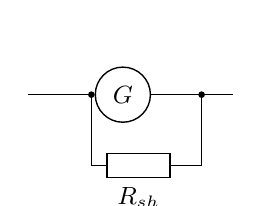
\begin{tikzpicture}[x=1cm,y=1cm,line width=0.5pt,>=Stealth,font=\small]
\draw (0,0)--(0.8,0); \draw[fill=white] (1.2,0) circle(0.35) node{$G$}; \draw (1.55,0)--(2.6,0); \draw (0.8,0)--(0.8,-0.9)--(1.0,-0.9);
\draw[fill=white] (1.0,-1.05) rectangle (1.8,-0.75); \node[below] at (1.4,-1.05) {$R_{sh}$}; \draw (1.8,-0.9)--(2.2,-0.9)--(2.2,0);
\fill (0.8,0) circle(1.2pt) (2.2,0) circle(1.2pt);
\end{tikzpicture}\end{center}
\noindent\textbf{33.}\ Galvanometrni 1 A gaça tokni ölçaydigan ampermetrga aylantiriş uçun şunt qarşiligini ($\Omega$) toping.\par
\noindent\textbf{34.}\ Galvanometrni 10 V gaça kuçlanişni ölçaydigan voltmetrga aylantiriş uçun ketma-ket ulanadigan qöşimça qarşilikni ($\Omega$) toping.\par
\noindent\textbf{35.}\ Hosil bölgan voltmetrning içki qarşiligini ($\Omega$) toping.\par
\noindent Variantlar: A) 0,99;\quad B) 1;\quad C) 100;\quad D) 901;\quad E) 990;\quad F) 1000\par\smallskip
\noindent\colorbox{gray!12}{\parbox{\dimexpr\linewidth-2\fboxsep}{\textbf{Javob: 33--B) 1; 34--D) 901; 35--F) 1000}}}\par\smallskip
\noindent\textit{Yechim.}\ Şunt: $I_gR_g=(I-I_g)R_s$,\par
\[R_s=\frac{0{,}01\cdot99}{1-0{,}01}=1\ \Omega.\]
Voltmetr: töliq qarşilik $R_V=U/I_g=10/0{,}01=1000\ \Omega$, qöşimça qarşilik $R_q=1000-99=901\ \Omega$. Voltmetrning içki qarşiligi $1000\ \Omega$.\par\par\medskip\hrule\medskip
\Needspace{12\baselineskip}\noindent\textbf{36.}\ Uzunligi 4 m, massasi 20 kg bölgan bir jinsli taxta uçlari bilan ikkita tayançga qöyilgan. Taxtaning çap uçidan 1 m masofada massasi 60 kg bölgan odam turibdi. $g=10$ m/s$^2$.\par
\noindent\hspace*{4mm}a)\ Çap tayançning taxtaga ta’sir kuçini (N) toping.\par
\noindent\hspace*{4mm}b)\ Öng tayançning taxtaga ta’sir kuçini (N) toping.\par
\noindent\colorbox{gray!12}{\parbox{\dimexpr\linewidth-2\fboxsep}{\textbf{Javob: a)\ 550;\quad b)\ 250}}}\par\smallskip
\noindent\textit{Yechim.}\ Öng tayançga nisbatan momentlar: $N_1\cdot4=200\cdot2+600\cdot3$, $N_1=550$ N. Kuçlar muvozanati: $N_2=800-550=250$ N.\par\par\medskip\hrule\medskip
\Needspace{12\baselineskip}\noindent\textbf{37.}\ Yer sirtidan 35 m balandlikdan jism tik yuqoriga 30 m/s tezlik bilan otildi. $g=10$ m/s$^2$.\par
\noindent\hspace*{4mm}a)\ Jismning Yer sirtidan eng katta kötariliş balandligini (m) toping.\par
\noindent\hspace*{4mm}b)\ Jism otilgandan neça sekunddan keyin Yerga tuşadi?\par
\noindent\colorbox{gray!12}{\parbox{\dimexpr\linewidth-2\fboxsep}{\textbf{Javob: a)\ 80;\quad b)\ 7}}}\par\smallskip
\noindent\textit{Yechim.}\ Otiliş nuqtasidan kötariliş $v^2/2g=45$ m, eng katta balandlik $35+45=80$ m. Kötariliş 3 s, 80 m dan tuşiş $\sqrt{2\cdot80/10}=4$ s. Jami $7$ s.\par\par\medskip\hrule\medskip
\Needspace{12\baselineskip}\noindent\textbf{38.}\ Massasi 2 kg bölgan şar 6 m/s tezlik bilan harakatlanib, tinç turgan 4 kg massali şarga urildi. Uriliş noelastik.\par
\noindent\hspace*{4mm}a)\ Urilişdan keyingi şarlarning umumiy tezligini (m/s) toping.\par
\noindent\hspace*{4mm}b)\ Urilişda ajralib çiqqan issiqlik miqdorini (J) toping.\par
\noindent\colorbox{gray!12}{\parbox{\dimexpr\linewidth-2\fboxsep}{\textbf{Javob: a)\ 2;\quad b)\ 24}}}\par\smallskip
\noindent\textit{Yechim.}\ \[u=\frac{m_1v}{m_1+m_2}=\frac{12}{6}=2\ \text{m/s},\qquad Q=\frac{2\cdot36}{2}-\frac{6\cdot4}{2}=36-12=24\ \text{J}.\]\par\medskip\hrule\medskip
\Needspace{12\baselineskip}\noindent\textbf{39.}\ 2 mol bir atomli ideal gaz 50 K ga qizdirildi. $R=8{,}31$ J/(mol$\cdot$K).\par
\noindent\hspace*{4mm}a)\ Qizdiriş özgarmas hajmda bölsa, gazga berilgan issiqlik miqdorini (J) toping.\par
\noindent\hspace*{4mm}b)\ Qizdiriş özgarmas bosimda bölsa, gazga berilgan issiqlik miqdorini (J) toping.\par
\noindent\colorbox{gray!12}{\parbox{\dimexpr\linewidth-2\fboxsep}{\textbf{Javob: a)\ 1246,5;\quad b)\ 2077,5}}}\par\smallskip
\noindent\textit{Yechim.}\ $Q_V=\frac32\nu R\Delta T=1{,}5\cdot2\cdot8{,}31\cdot50=1246{,}5$ J; $Q_p=\frac52\nu R\Delta T=2077{,}5$ J.\par\par\medskip\hrule\medskip
\Needspace{12\baselineskip}\noindent\textbf{40.}\ Qörğoşin öq 260 m/s tezlik bilan devorga urilib töxtadi. Öq kinetik energiyasining 50\% i uni isitişga ketdi. $c_{qo‘rg‘oshin}=130$ J/(kg$\cdot$K).\par
\noindent\hspace*{4mm}a)\ Öq temperaturasi neça kelvinga ortadi?\par
\noindent\hspace*{4mm}b)\ Öqning dastlabki temperaturasi 27 $^\circ$C bölsa, uning oxirgi temperaturasini ($^\circ$C) toping.\par
\noindent\colorbox{gray!12}{\parbox{\dimexpr\linewidth-2\fboxsep}{\textbf{Javob: a)\ 130;\quad b)\ 157}}}\par\smallskip
\noindent\textit{Yechim.}\ \[0{,}5\cdot\frac{mv^2}{2}=cm\Delta T\ \Rightarrow\ \Delta T=\frac{0{,}25v^2}{c}=\frac{0{,}25\cdot67\,600}{130}=130\ \text{K}.\]
Oxirgi temperatura $27+130=157\ ^\circ$C.\par\par\medskip\hrule\medskip
\Needspace{12\baselineskip}\noindent\textbf{41.}\ Induktivligi 0,2 H bölgan ğaltakdan 3 A tok ötmoqda.\par
\noindent\hspace*{4mm}a)\ Ğaltak magnit maydonining energiyasini (J) toping.\par
\noindent\hspace*{4mm}b)\ Tok 0,05 s davomida bir tekis nolgaça kamayganda hosil böladigan özinduksiya EYuKni (V) toping.\par
\noindent\colorbox{gray!12}{\parbox{\dimexpr\linewidth-2\fboxsep}{\textbf{Javob: a)\ 0,9;\quad b)\ 12}}}\par\smallskip
\noindent\textit{Yechim.}\ \[W=\frac{LI^2}{2}=\frac{0{,}2\cdot9}{2}=0{,}9\ \text{J},\qquad \mathcal E=L\frac{\Delta I}{\Delta t}=0{,}2\cdot\frac{3}{0{,}05}=12\ \text{V}.\]\par\medskip\hrule\medskip
\Needspace{12\baselineskip}\noindent\textbf{42.}\ Bir xil ölçamli ikkita metall şarçaning zaryadlari $+6$ nC va $-2$ nC. Şarçalar bir-biriga tekkizilib, söngra 3 cm masofaga uzoqlaştirildi. $k=9\cdot10^9$ N$\cdot$m$^2$/C$^2$.\par
\noindent\hspace*{4mm}a)\ Tekkizilgandan keyin har bir şarçaning zaryadini (nC) toping.\par
\noindent\hspace*{4mm}b)\ Şarçalarning özaro ta’sir kuçini ($\mu$N) toping.\par
\noindent\colorbox{gray!12}{\parbox{\dimexpr\linewidth-2\fboxsep}{\textbf{Javob: a)\ 2;\quad b)\ 40}}}\par\smallskip
\noindent\textit{Yechim.}\ Umumiy zaryad $6-2=4$ nC teng bölinadi: har biriga 2 nC.\par
\[F=k\frac{q^2}{r^2}=9\cdot10^9\cdot\frac{4\cdot10^{-18}}{9\cdot10^{-4}}=4\cdot10^{-5}\ \text{N}=40\ \mu\text{N}.\]\par\medskip\hrule\medskip
\Needspace{12\baselineskip}\noindent\textbf{43.}\ Yung tajribasida tirqişlar orasidagi masofa 0,5 mm, tirqişlardan ekrangaça masofa 2 m, yoruğlikning tölqin uzunligi 500 nm.\par
\noindent\hspace*{4mm}a)\ Qöşni yoruğ polosalar orasidagi masofani (mm) toping.\par
\noindent\hspace*{4mm}b)\ Markaziy maksimumdan uçinçi yoruğ polosagaça masofani (mm) toping.\par
\noindent\colorbox{gray!12}{\parbox{\dimexpr\linewidth-2\fboxsep}{\textbf{Javob: a)\ 2;\quad b)\ 6}}}\par\smallskip
\noindent\textit{Yechim.}\ \[\Delta x=\frac{\lambda L}{d}=\frac{5\cdot10^{-7}\cdot2}{5\cdot10^{-4}}=2\cdot10^{-3}\ \text{m}=2\ \text{mm}.\]
Uçinçi yoruğ polosa $3\Delta x=6$ mm da.\par\par\medskip\hrule\medskip
\Needspace{12\baselineskip}\noindent\textbf{44.}\ Proyeksion apparat balandligi 24 mm bölgan diapozitivning ekranda balandligi 1,2 m bölgan tasvirini hosil qiladi. Ekran obyektivdan 5,1 m uzoqlikda.\par
\noindent\hspace*{4mm}a)\ Apparatning çiziqli kattalaştirişini toping.\par
\noindent\hspace*{4mm}b)\ Obyektivning fokus masofasini (cm) toping.\par
\noindent\colorbox{gray!12}{\parbox{\dimexpr\linewidth-2\fboxsep}{\textbf{Javob: a)\ 50;\quad b)\ 10}}}\par\smallskip
\noindent\textit{Yechim.}\ $\Gamma=\frac{1{,}2}{0{,}024}=50$. $f=5{,}1$ m, $d=f/\Gamma=0{,}102$ m.\par
\[F=\frac{df}{d+f}=\frac{0{,}102\cdot5{,}1}{5{,}202}=0{,}1\ \text{m}=10\ \text{cm}.\]\par\medskip\hrule\medskip
\Needspace{12\baselineskip}\noindent\textbf{45.}\ Elektron tinç holatdan 150 V potensiallar farqida tezlatildi. $m_e=9{,}1\cdot10^{-31}$ kg, $e=1{,}6\cdot10^{-19}$ C, $h=6{,}6\cdot10^{-34}$ J$\cdot$s.\par
\noindent\hspace*{4mm}a)\ Elektron impulsini ($10^{-24}$ kg$\cdot$m/s) toping.\par
\noindent\hspace*{4mm}b)\ Elektronning de Broyl tölqin uzunligini (nm) toping.\par
\noindent\colorbox{gray!12}{\parbox{\dimexpr\linewidth-2\fboxsep}{\textbf{Javob: a)\ 6,61;\quad b)\ 0,1}}}\par\smallskip
\noindent\textit{Yechim.}\ \[p=\sqrt{2meU}=\sqrt{2\cdot9{,}1\cdot10^{-31}\cdot1{,}6\cdot10^{-19}\cdot150}\approx6{,}61\cdot10^{-24}\ \text{kg}\cdot\text{m/s},\]
\[\lambda=\frac{h}{p}=\frac{6{,}6\cdot10^{-34}}{6{,}61\cdot10^{-24}}\approx10^{-10}\ \text{m}=0{,}1\ \text{nm}.\]\par\medskip\hrule\medskip
\end{document}